\section{Interacción con el blanco}
\subsection{¿Que es una imagen SAR?}
\begin{frame}{\secname : \subsecname}
  \begin{columns}[t]
    \begin{column}{0.5\textwidth}
     \begin{block}{SAR}
       \begin{itemize}
         \item Una imagen SAR es un mapa de reflectividad.
         \item Indica cuanta energía es devuelta al sensor.
         \item La cantidad de energía retrodispersaada depende de la geometría del blanco y su conductividad eléctrica.
         \item Las zonas oscurar y brillantes son zonas de baja y alta reflectividad.
       \end{itemize}
     \end{block}
    \end{column}
    \begin{column}{0.5\textwidth}  %%<--- here
        \begin{figure}
          \centering
          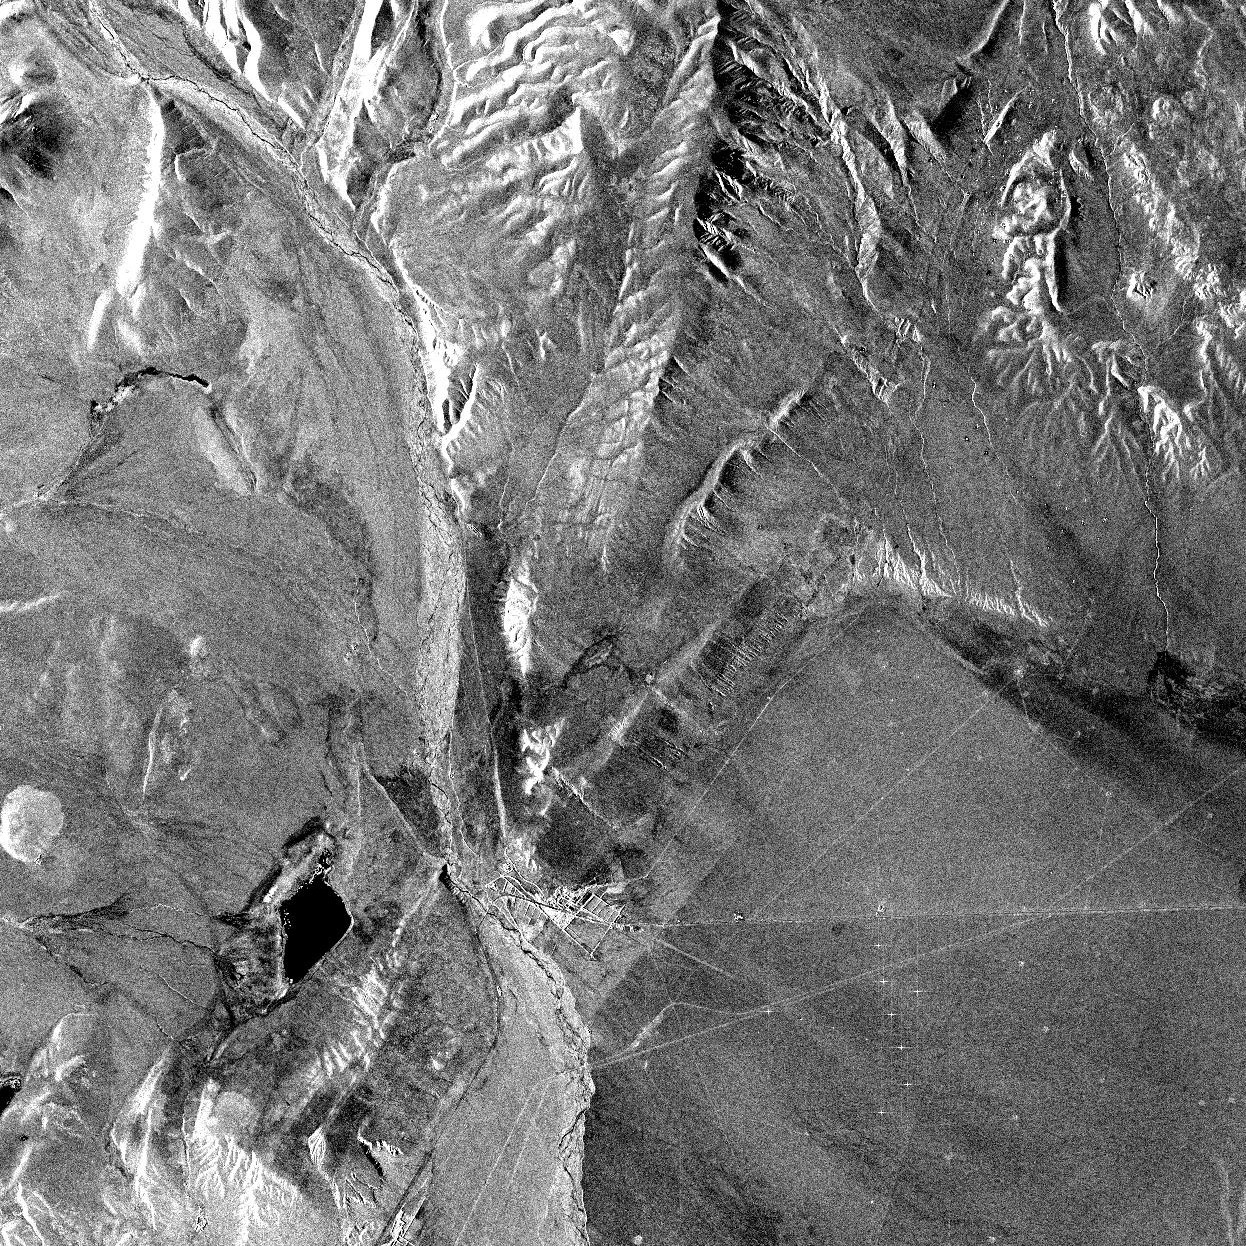
\includegraphics[width=\textwidth]{fig:sar.jpg}
          \caption{}
          \label{}
        \end{figure}
    \end{column}
    \end{columns}
\end{frame}
%--- Next Frame ---%

\begin{frame}{\secname : \subsecname}
    \begin{figure}
      \centering
      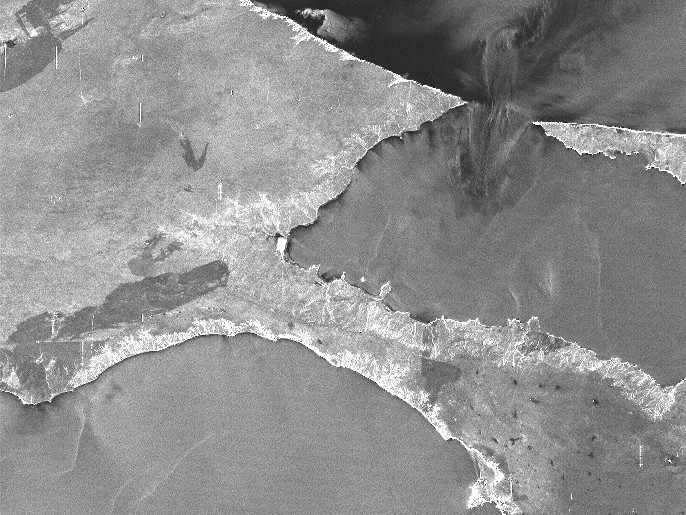
\includegraphics[width=0.6\textwidth]{fig:sar2.jpg}
      \caption{}
      \label{}
    \end{figure}
\end{frame}
%--- Next Frame ---%

\subsection{Mecanismos de scattering}

\begin{frame}{\secname : \subsecname}
    \begin{figure}
      \centering
      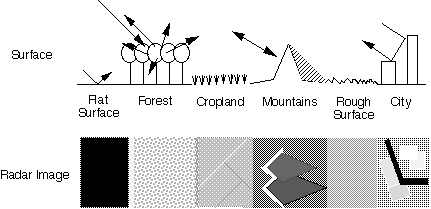
\includegraphics[width=0.6\textwidth]{fig:rebotes.png}
      \caption{}
      \label{}
    \end{figure}
\end{frame}
%--- Next Frame ---%

\begin{frame}{\secname : \subsecname}
    \begin{figure}
      \centering
      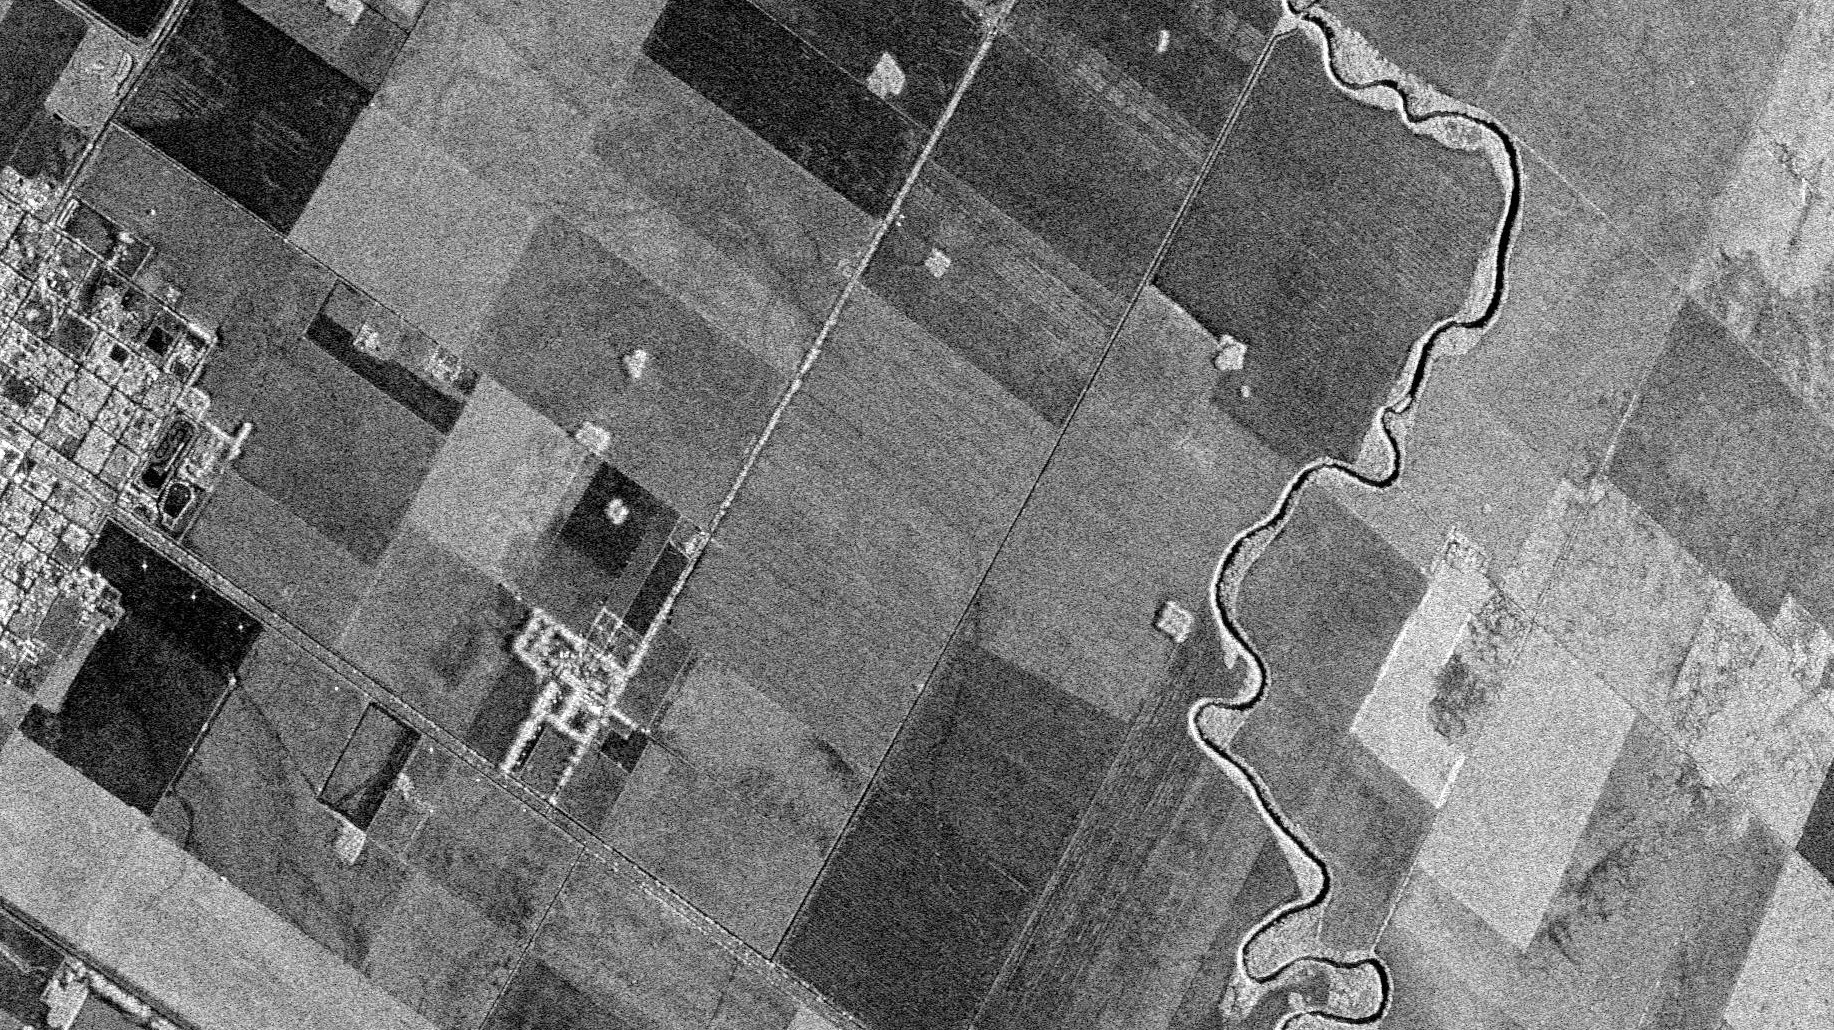
\includegraphics[width=0.6\textwidth]{fig:rebotes2.jpg}
      \caption{}
      \label{}
    \end{figure}
\end{frame}
%--- Next Frame ---%

\begin{frame}{\secname : \subsecname}
    \begin{figure}
      \centering
      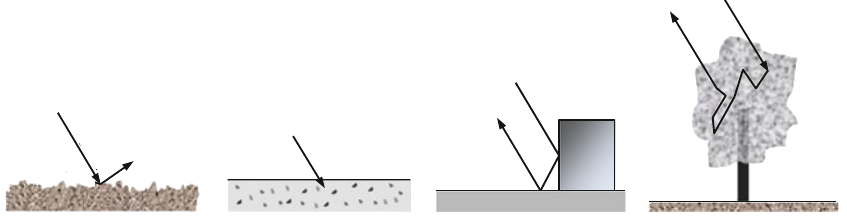
\includegraphics[width=0.5\textwidth]{fig:interacciones.png}
      \caption{}
      \label{}
    \end{figure}
\end{frame}
%--- Next Frame ---%

\begin{frame}{\secname : \subsecname}
    \begin{figure}
    \centering
    \subfloat[Banda C ($5.7cm$)]{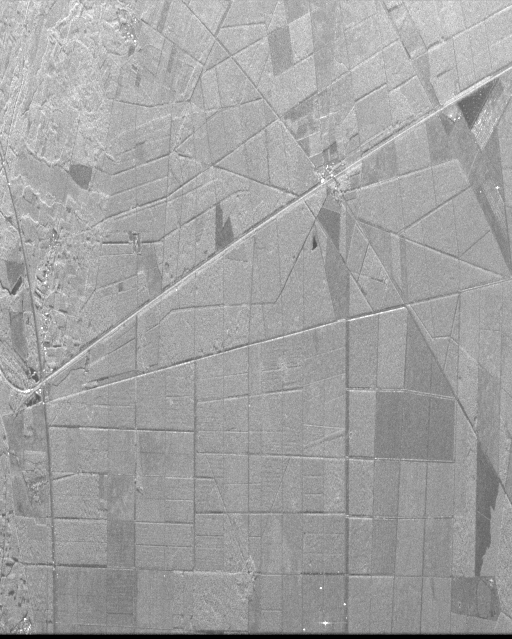
\includegraphics[width=0.2\textwidth]{fig:C.png}}\hspace{1cm}
    \subfloat[Banda L ($24cm$)]{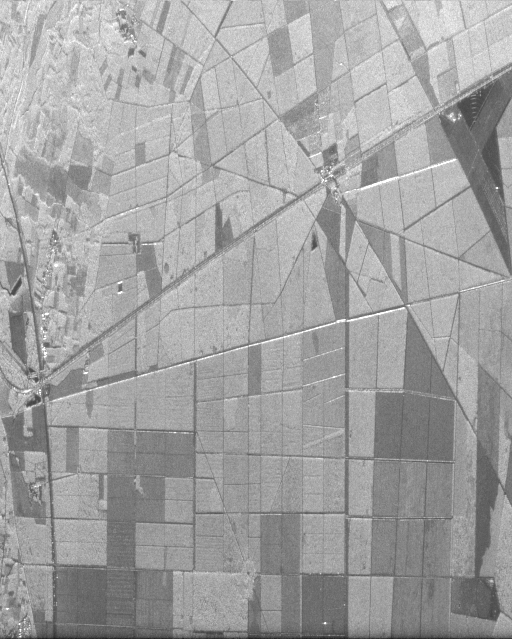
\includegraphics[width=0.2\textwidth]{fig:L.png}}\hspace{1cm}
    \subfloat[Banda P ($68cm$)]{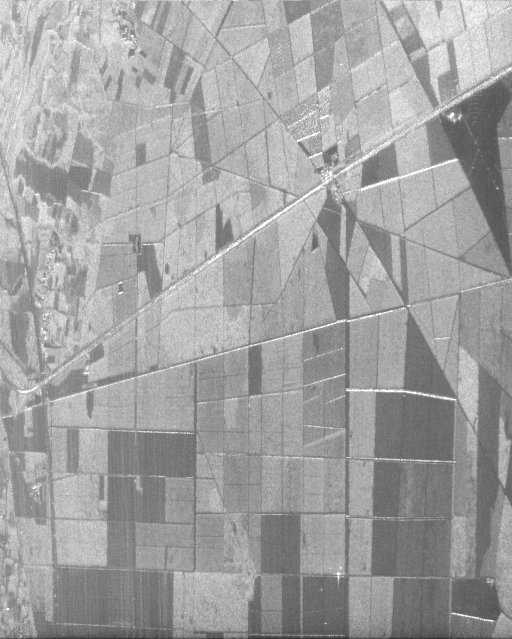
\includegraphics[width=0.2\textwidth]{fig:P.png}}
    \end{figure}
\end{frame}
%--- Next Frame ---%

\subsection{Resolución}
\begin{frame}{\secname : \subsecname}
    \begin{figure}
      \centering
      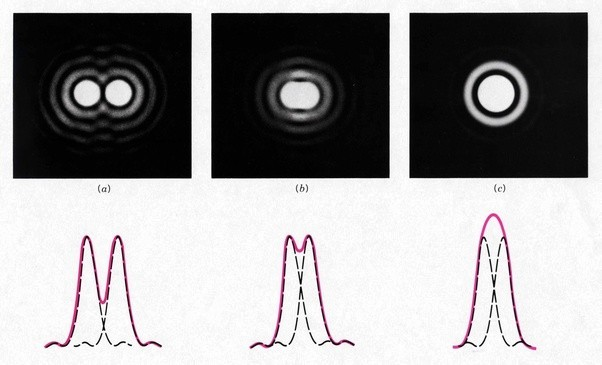
\includegraphics[width=0.5\textwidth]{fig:bandwidth.jpg}
      \caption{}
      \label{}
    \end{figure}
\end{frame}
%--- Next Frame ---%


\begin{frame}{\secname : \subsecname}
    \begin{figure}
      \centering
      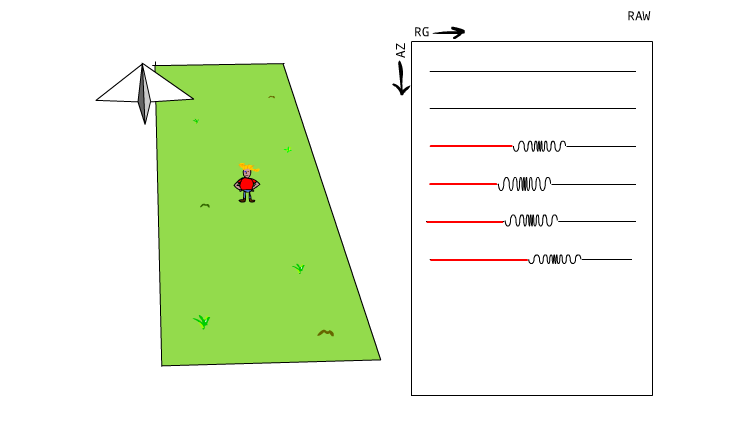
\includegraphics[width=0.5\textwidth]{fig:rgaz.png}
      \caption{}
      \label{}
    \end{figure}
\end{frame}
%--- Next Frame ---%

\begin{frame}{\secname : \subsecname}
  \begin{columns}
    \begin{column}{0.5\textwidth}
     \begin{block}{Resolución en rango}
      \begin{equation}
        \rho_{RG} = \frac{c}{2B}
      \end{equation}
     \end{block}
    \end{column}
    \begin{column}{0.5\textwidth}  %%<--- here
      \begin{block}{Resolución en azymuth}
        \begin{equation}
          \rho_{AZ} = \frac{L}{2}
        \end{equation}
      \end{block}
    \end{column}
    \end{columns}
    con $c$ la velocidad de la luz, $B$ el \emph{bandwidth} del sistema y $L$ la longitud de la antena.
\end{frame}
%--- Next Frame ---%

\subsection{Distorciones geométricas}

\begin{frame}{\secname : \subsecname}
  \begin{columns}[t]
    \begin{column}{0.5\textwidth}
      \begin{figure}
        \centering
        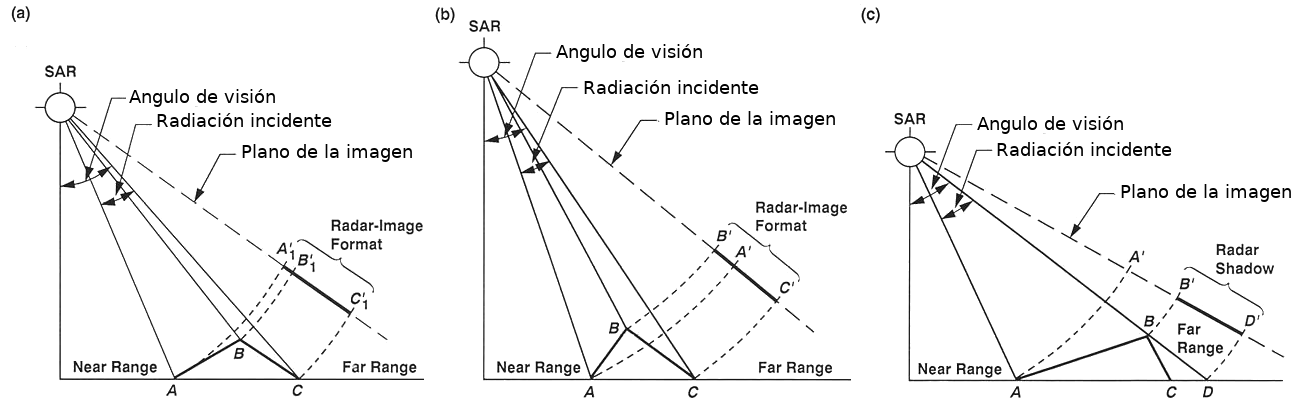
\includegraphics[width=\textwidth]{fig:dist.png}
        \caption{}
        \label{}
      \end{figure}
    \end{column}
    \begin{column}{0.5\textwidth}  %%<--- here
        \begin{figure}
          \centering
          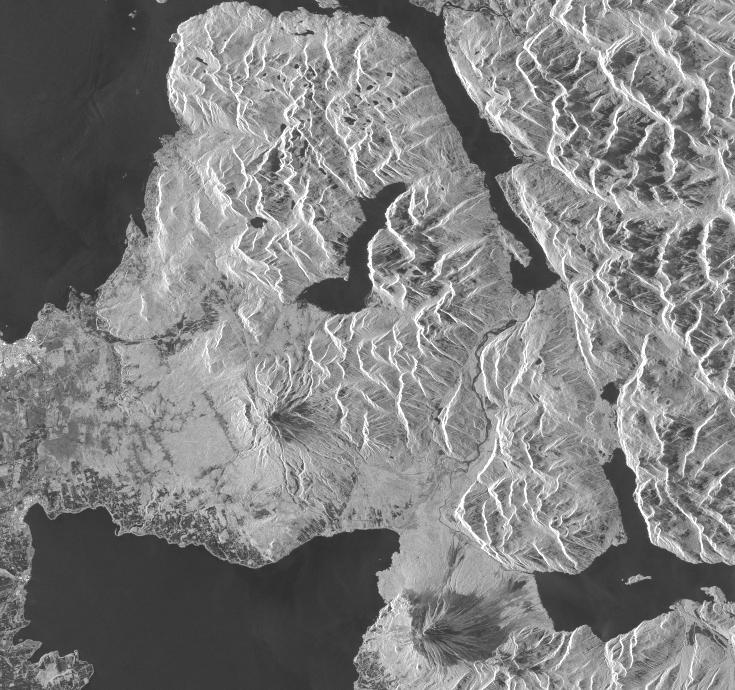
\includegraphics[width=\textwidth]{fig:dist2.jpg}
          \caption{}
          \label{}
        \end{figure}
    \end{column}
    \end{columns}
\end{frame}
%--- Next Frame ---%

\begin{frame}{\secname : \subsecname}
    \begin{figure}
      \centering
      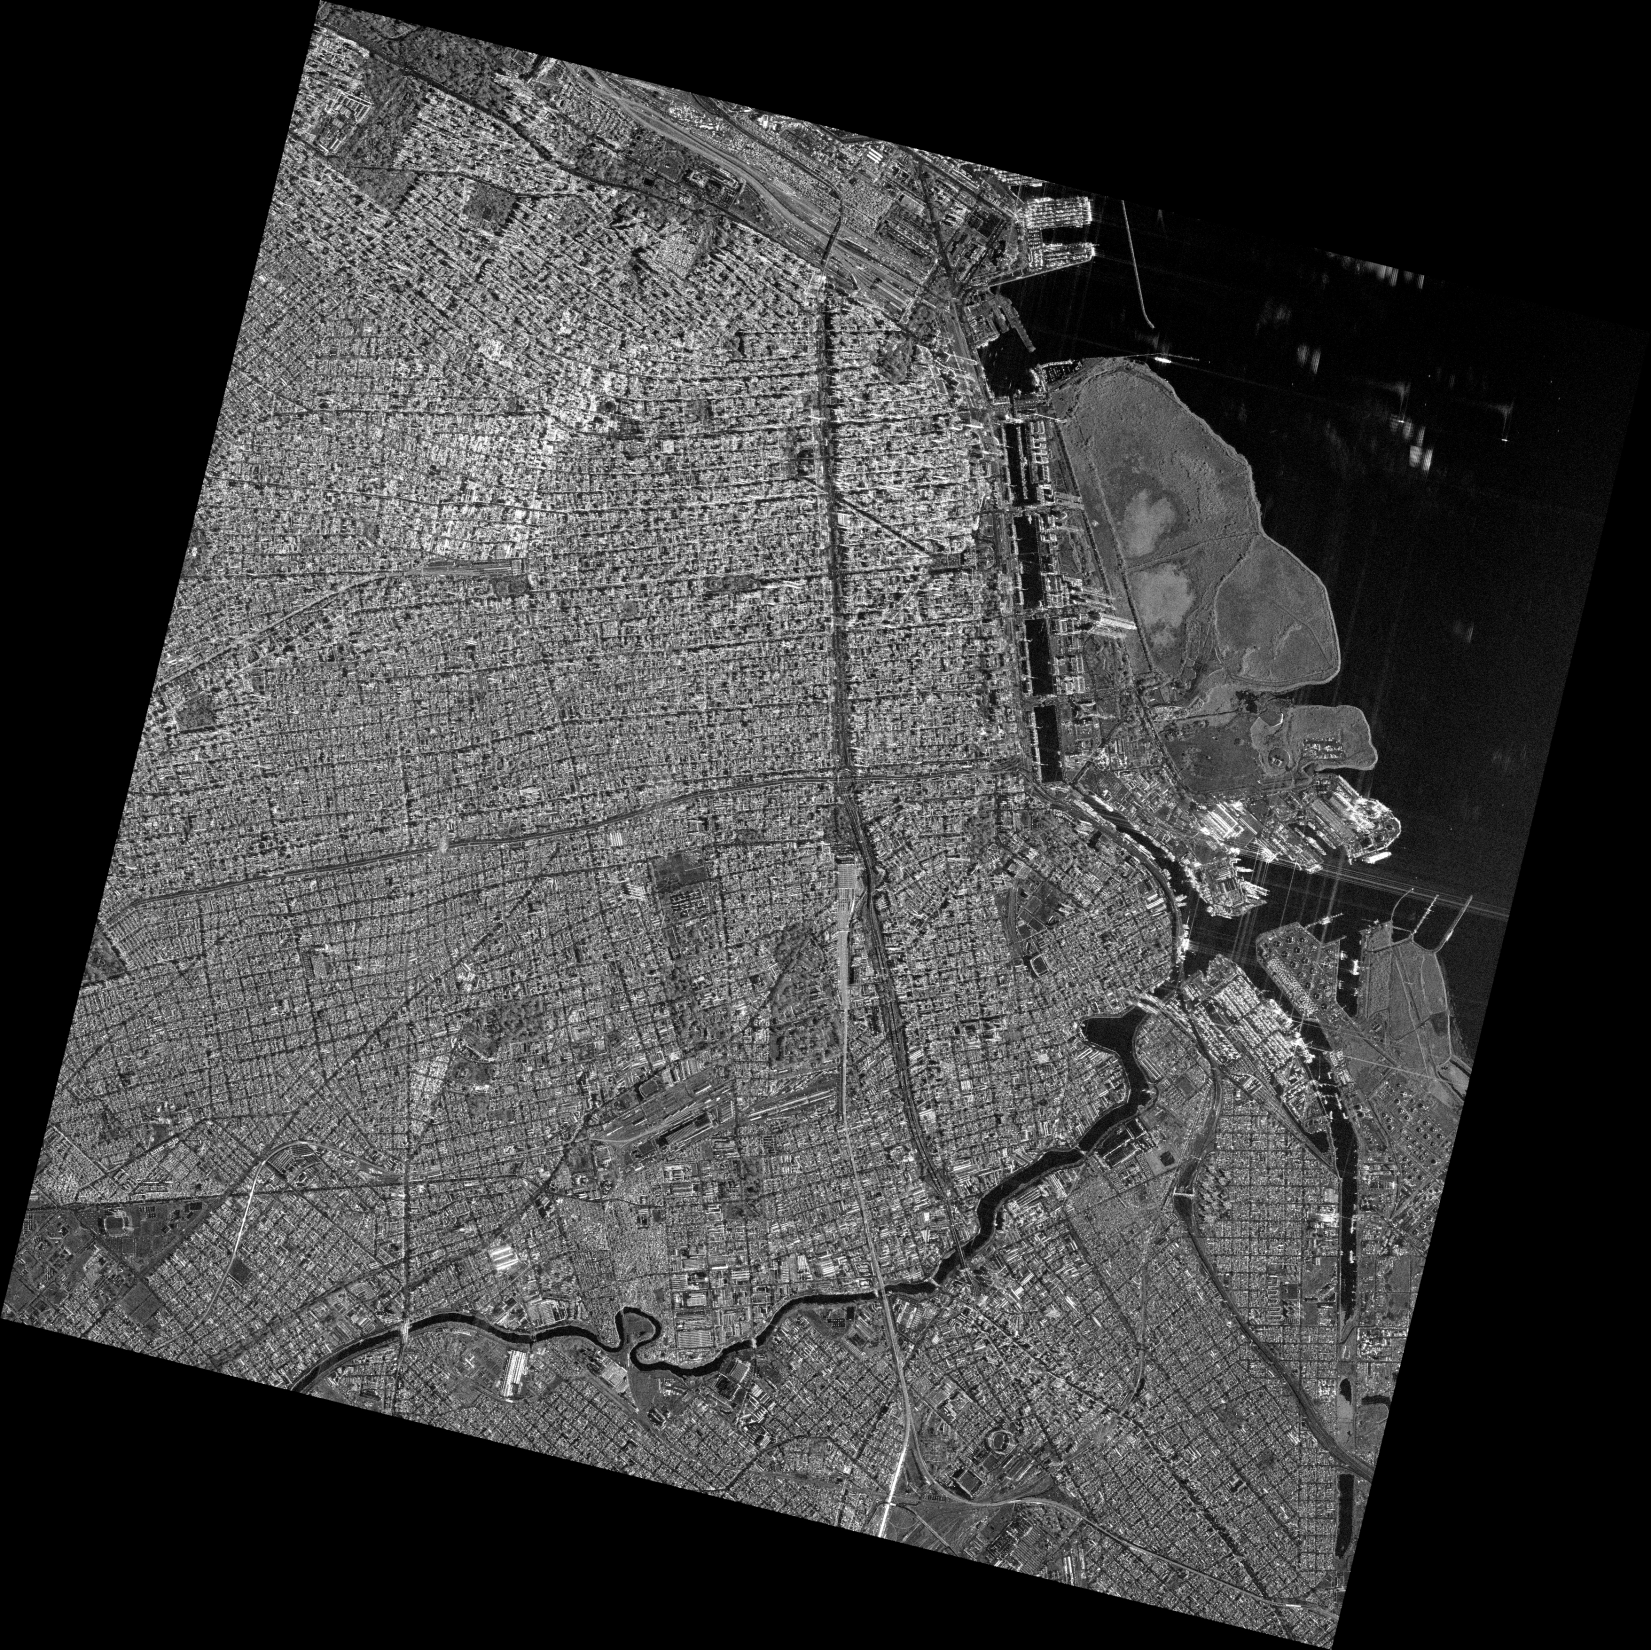
\includegraphics[width=0.5\textwidth]{fig:ba.png}
      \caption{}
      \label{}
    \end{figure}
\end{frame}
%--- Next Frame ---%

\begin{frame}{\secname : \subsecname}
  \begin{columns}[t]
    \begin{column}{0.5\textwidth}
      \begin{figure}
        \centering
        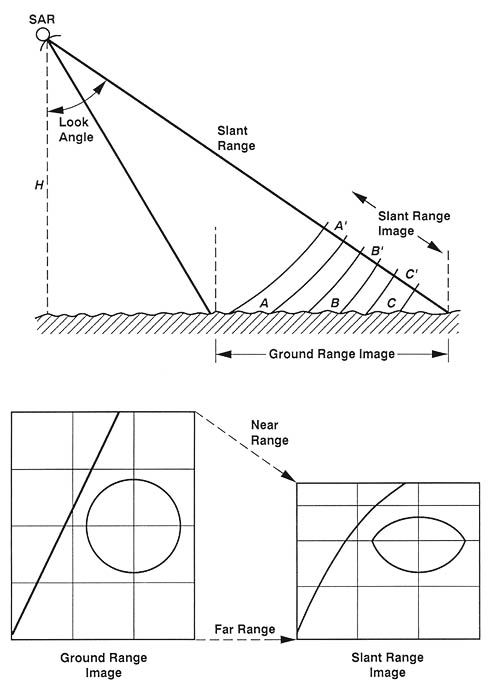
\includegraphics[height=0.7\textheight]{fig:slantground.png}
        \caption{}
        \label{}
      \end{figure}
    \end{column}
    \begin{column}{0.5\textwidth}  %%<--- here
        \begin{figure}

          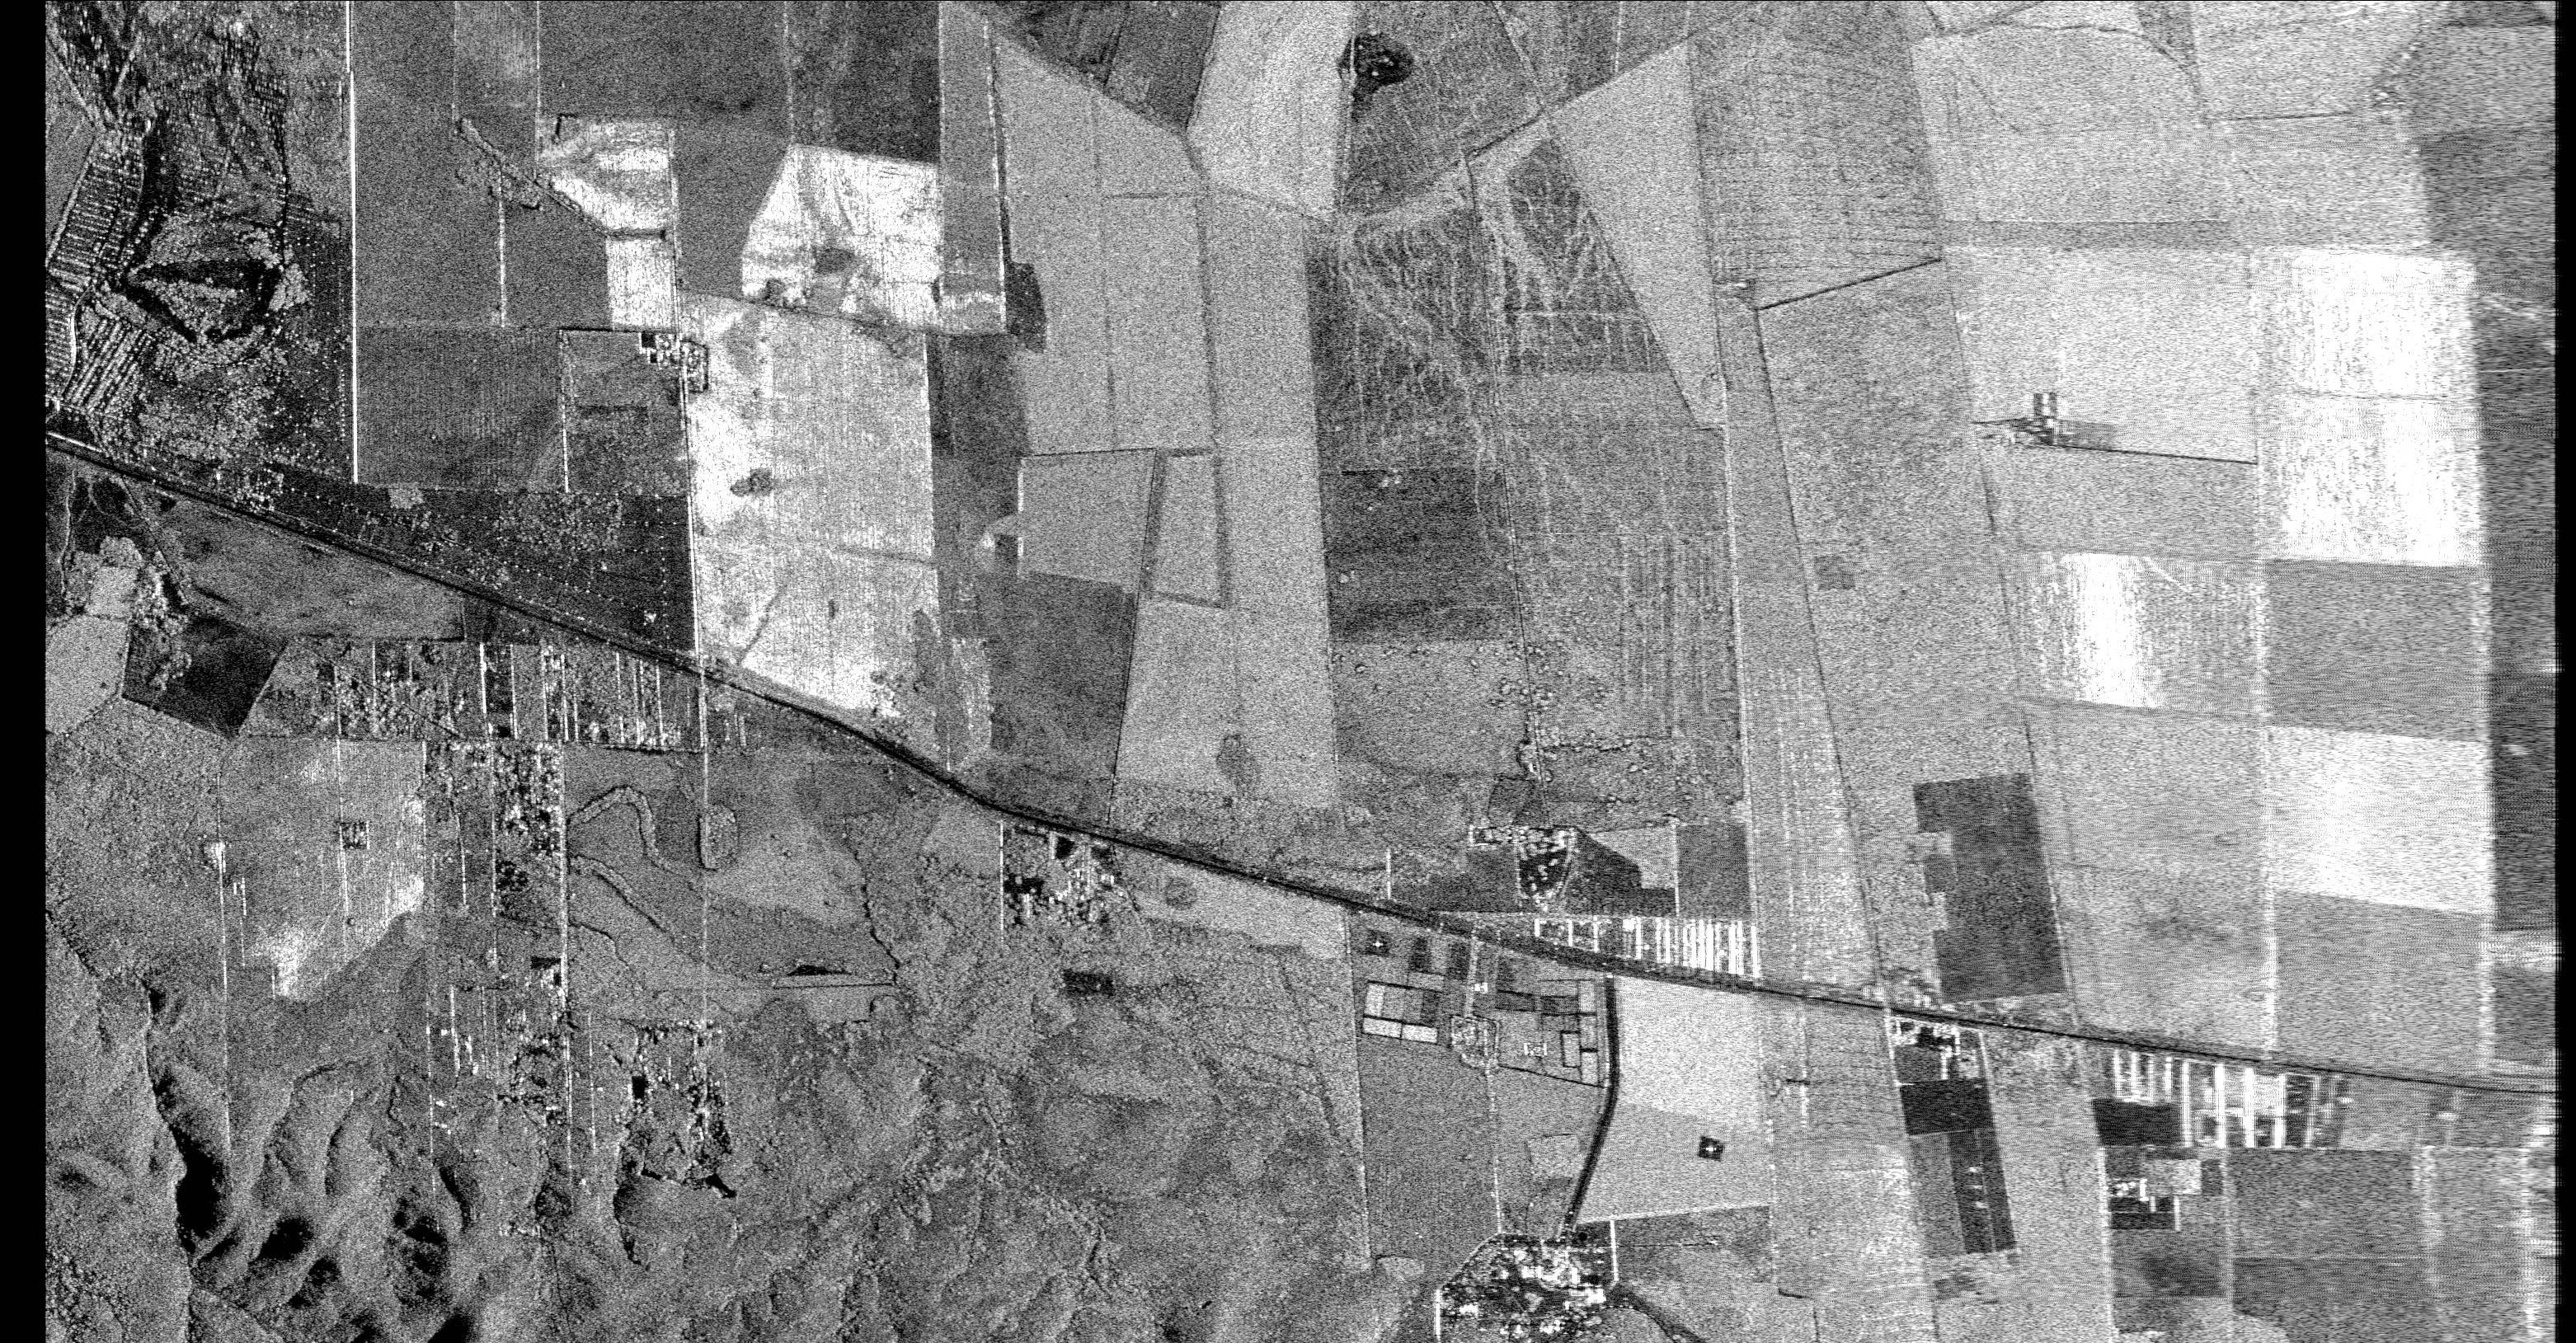
\includegraphics[height=0.2\textwidth]{fig:slant.jpg}\\
          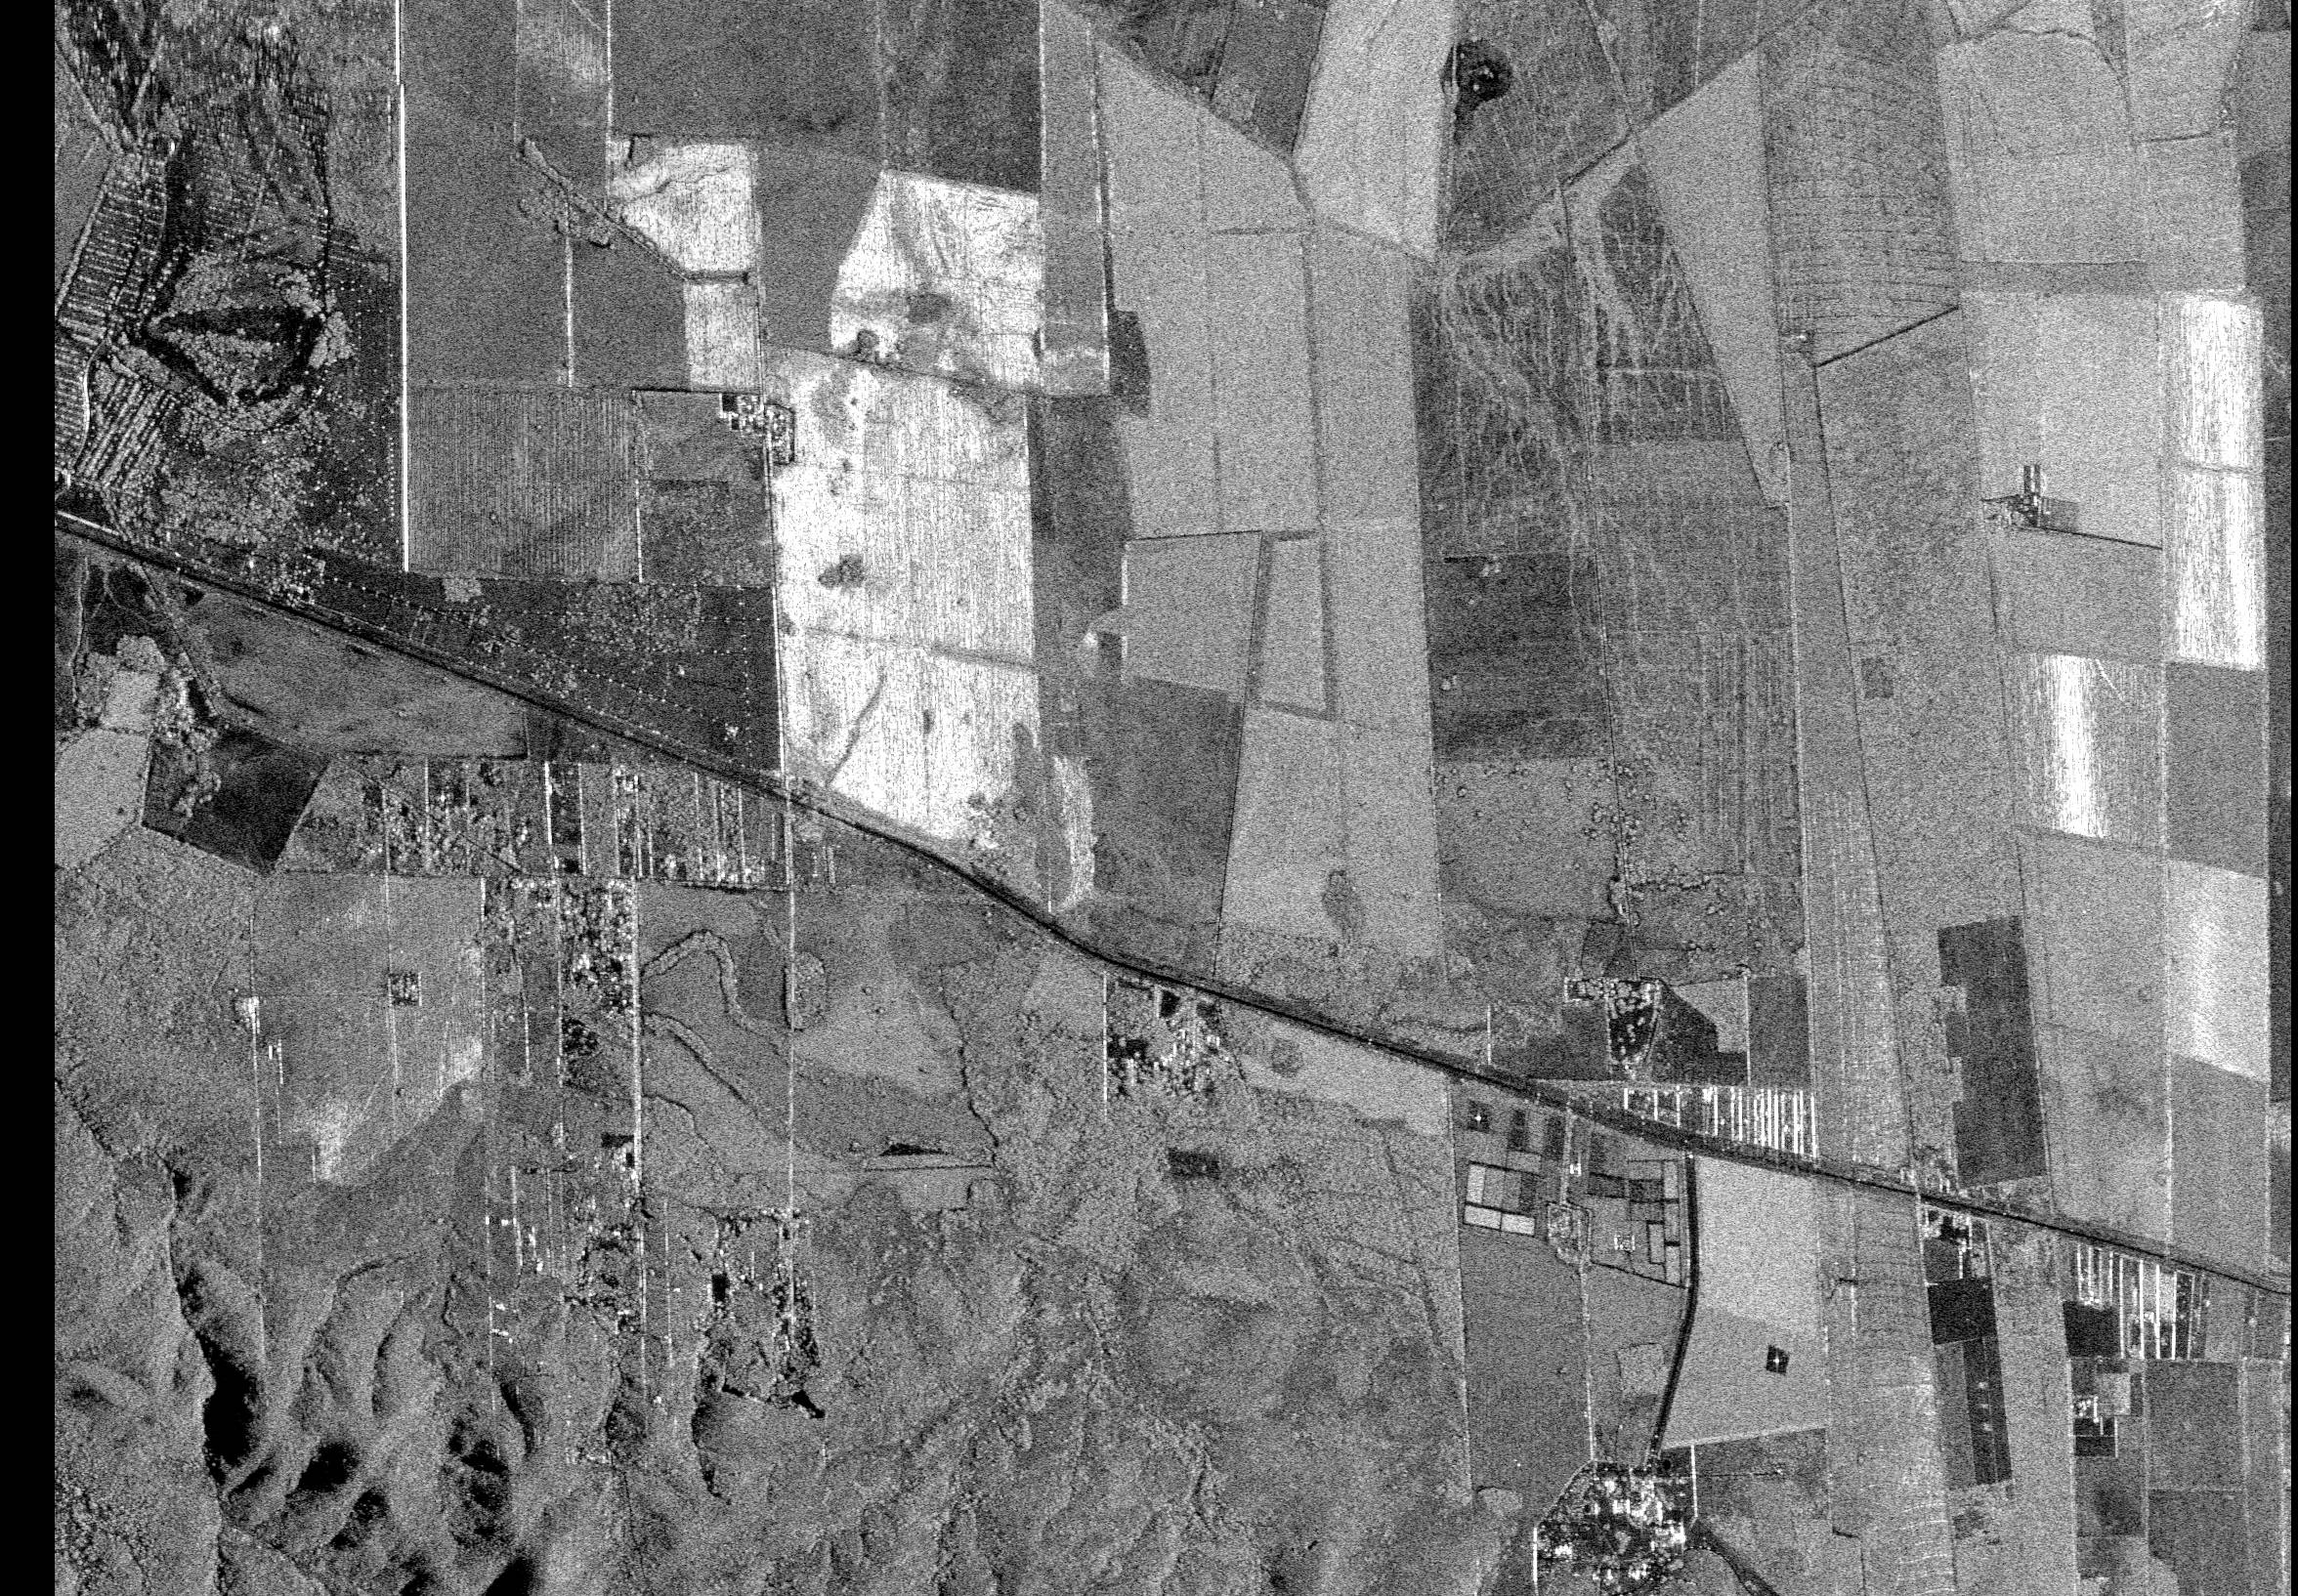
\includegraphics[height=0.2\textwidth]{fig:ground.jpg}
          \caption{}
          \label{}
        \end{figure}
    \end{column}
    \end{columns}
\end{frame}
%--- Next Frame ---
